Prim算法和Kruskal算法都属于最小生成树算法.
\subsubsection{最小生成树}
\label{sub:MST}
\paragraph*{生成树} 设一个网络表示为无向连通带权图$G=(V, E)$, E中每条边$(u,
	v)$的权为$w(u, v)$. 如果G的子图G'是一棵包含G的所有顶点的树,
则称G'为G的生成树.\par

\paragraph*{生成树的成本} 生成树上各边权的总和.\par

\paragraph*{G的最小生成树} 在G的所有生成树中, 耗费最小的生成树.

\paragraph{最小生成树性质}
基于贪心选择策策略, 构造最小生成树算法:
\begin{enumerate}
	\item Kruskal算法
	\item Prim算法
\end{enumerate}

这2个算法的贪心选择方法不同, 但是都利用了最小生成树(MST)性质:\par
设$G=(V, E)$是连通带权图, 顶点集U是V的真子集. 如果:
\begin{enumerate}
	\item $(u,v)\in E$为横跨点集U和V-U的边, 即$u\in U, v\in V-U$, 并且
	\item 在所有这样的边中, $(u, v)$的权$w(u, v)$ 最小,
	      则一定存在G的一颗最小生成树, 它以$(u, v)$为其中一条边, 即$(u,
		      v)$出现在最小生成树中.
\end{enumerate}

\paragraph{最小生成树性质证明}
使用反证法.\par
假设对G的任意一个最小生成树T, 针对点集U和V-U, $(u,v)\in
	E$为横跨这两个点集的最小权边, T不包含该最小权边(u,v), 但是T包含u和v.\par

将(u,v)添加到树T中, 树T变为含回路的子图,
且该回路上有一条不同于(u,v)的边$(u',v'), u'\in U, v'\in V-U$. 将(u',v')删去,
得到另一个树T', 即树T'是通过将T中的边(u', v')替换为(u,v)得到的.\par

由于这两条边的耗费满足$w(u,v)\leq w(u',v')$,
因此用较小耗费的边(u,v)替换后得到的树T'的耗费更小, 即
\begin{equation}
	Cost(T')\leq Cost(T)
\end{equation}
这与T是任意最小生成树的假设矛盾.\par
故MST的性质得证.

\subsubsection{算法类别}
Prim算法属于贪心算法.

\subsubsection{问题描述}
设$G=(V,E)$是连通带权图, $V=\{1,2,\dots,n\}$. 求节~\ref{sub:MST}所描述的最小生成树.

\subsubsection{Prim算法的基本思路}
\begin{enumerate}
	\item 首先置顶点集合$S=\{1\}$
	\item 当S是V的真子集的时候, 作如下贪心选择: 选取满足条件$i\in S, j\in V-S$,
	      且$w(i,j)$最小的边(i,j), 将顶点j添加到S中, 边(i,j)添加到边集T中.
	\item 重复上述过程, 直到S=V为止. 此时边集T就是一棵最小生成树.
\end{enumerate}
该算法的时间复杂度为$O(N^2)$.


\subsubsection{Prim算法的正确性证明}
即证明: 如果S是Prim算法从图$G=(V,E)$中选择的生成树, 则S是G的最小生成树.\par
证明: 用反证法. 假设S不是权重和最小的.
设$ES=(e_1,e_2,\cdots,e_{n-1})$是由Prim算法按顺序选择的边序列,
U为ES生成的最小生成树, 其中的边与ES有尽可能长的重合前缀.\par

设$e_i=(x,y)$为Prim算法选出来的边序列中第一条不在U中的边,
W为在$(x,y)$选择之前的点集合.
易知U包含边$e_1,e_2,\cdots,e_{i-1}$但不包含边$e_{i}$.\par

\begin{wrapfigure}{r}{width=0.5\textwidth}
	\begin{center}
		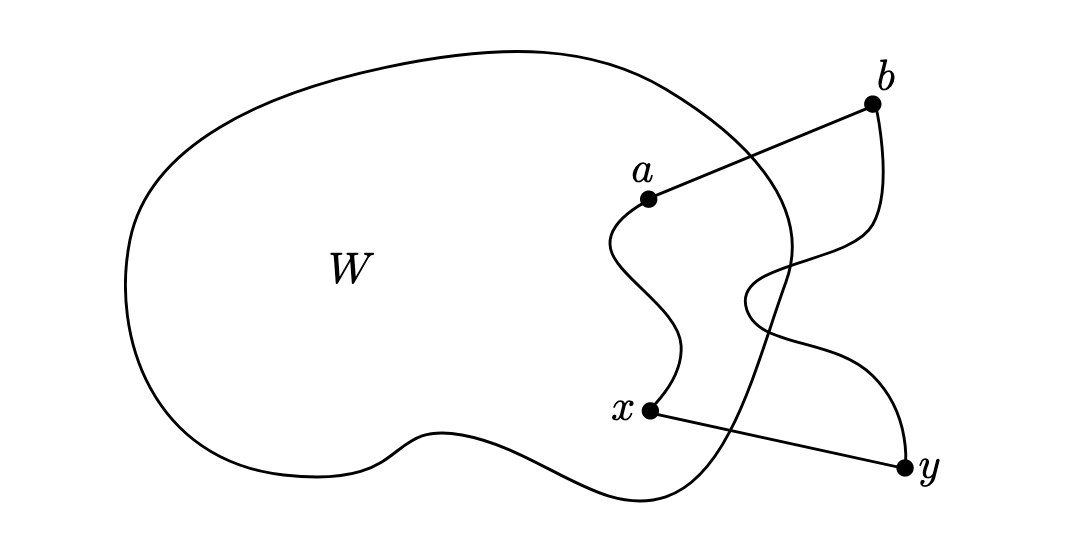
\includegraphics[width=0.48\textwidth]{prim-proof.png}
	\end{center}
	\label{fig:prim-proof}
\end{wrapfigure}

在U中一定有一条路径$x\arrowvert y\in U$, 使得(a,b)是这条路径上的第一条边,
且一个顶点在W中, 另一个顶点在W外.

设边集$T=U+\{(x,y)\}-\{(a,b)\}$, 其中(x,y)是前面提到的ES中的边.
注意到T是图G的一个生成树. 考虑边(x,y)和(a,b)的权重的三种可能情况:
\begin{description}
	\item[Case 1]  $w(a,b) > w(x,y)$. 在这种情况下, 创建T的时候树的权重总和减小,
		因此$w(T) < w(U)$. 这与U是最小生成树矛盾.
	\item[Case 2] $w(a,b) = w(x,y)$. 在这种情况下$w(T)=w(U)$, 因此T也是最小生成树.
		此外, 由于Prim算法还没有选择边(a,b), 这条边不可能在$e_1,e_2,\cdots,
			e_{i-1}$中. 这说明T包含边$e_1,e_2,\cdots,e_i$, 即T中含有ES的前缀比U的更长,
		这与U的定义矛盾.
	\item[Case 3] $w(a,b)<w(x,y)$. 在这种情况下, 因为w(a,b)更小,
		Prim算法在这一步会选择边$(a,b)$, 矛盾.
\end{description}
综上, Prim选出的是最小生成树. 至此, 完成了Prim算法的正确性证明.

\subsubsection{关键函数及代码段的描述}
\begin{algorithm}
	\begin{algorithmic}{1}
		\Require $(G, w, r)$
		\For{each u \in G.V}
		\State $u.distance = \infty$
		\EndFor
		\State r.distance = 0
		\State Q = G.V
		\While{$Q \neq \emptyset$}
		\State $u = Extract-Min(Q)$
		\For{each v \in G.Adj[u]}
		\If{v\in Q and w(u, v) < v.distance}
		\State v.distance = w(u,v)
		\EndIf`
		\EndFor
		\EndWhile
	\end{algorithmic}
\end{algorithm}
其核心代码实现如下:

% TODO: Add code here

\subsubsection{算法时间及空间复杂性分析}
\paragraph{空间复杂度分析}
使用邻接表存图, 空间复杂度为$O(V+E)$. 使用二叉最小堆维护顶点集合,
空间复杂度为$O(V)$.

\paragraph{时间复杂度分析}
由于使用了二叉最小堆, 堆的初始化开销为$O(|V|lg|V|)$.
对源进行Decrease-Key开销为$O(lg|V|)$. while循环中,
|V|的Extract-Min操作开销$O(|V|lg|V|)$. $\leq |E|$
Decrease-Key开销为$O(|E|lg|E|$. 总计为
\begin{align}
	T = & O(|V|\lg |V|) + O(\lg |V|) + O(|V|\lg |V|) + O(|E|\lg |E|)  \nonumber \\
	=   & O(E \lg V) \nonumber
\end{align}
由于图G是联通的, 故$\lg |E| = \Theta (\lg |V|)$, 时间复杂度为$O(E\lg V)$.
